\documentclass[10pt]{article}

% Required packages
\usepackage{bm,bbm}
\usepackage{amsmath,amssymb,amsthm,cancel}
\usepackage{algorithm, algpseudocode}
\usepackage{minted, caption}



% Color references
\usepackage[
    colorlinks=true, citecolor=green, linkcolor=blue]{hyperref}

\newcommand{\homework}[2]{
	\noindent
    \begin{center}
    	\framebox{
        	\vbox{
            	% Course Title and Date
            	\hbox to \hsize { \textsc{ORIE 7390 - Special Topics in
				Mathematical Programming} \hfill \textsc{#1} }
                \vspace{4mm}
                % Title of handout/homework
                \hbox to \hsize { {\Large \hfill \textsc{#2} \hfill} }
                \vspace{1mm}
            }
        }
    \end{center}
}

\newenvironment{alglist}{\begin{list}{}{\setlength{\leftmargin}{1.5cm}
\setlength{\rightmargin}{0cm}\setlength{\itemsep}{1ex}\setlength{\parsep}{1ex}}}{\end{list}}

\newcommand{\problem}[3]
{\fbox{\parbox{6in}{{\bf #1}\begin{itemize}\item{\bf Input:} {#2} \item{\bf Goal:} {#3}\end{itemize}}}}

\usepackage{latex-macros}
\usepackage{todonotes}
\usepackage{tikz,pgfplots}
\pgfplotsset{compat=1.12}
\usepackage{algorithm, algpseudocode}
\usepackage[margin=1in]{geometry}
\usetikzlibrary{shapes.geometric}
%\usepackage{parskip}
\usepackage[capitalize]{cleveref}
\usepackage{exercise}

\usepackage{todonotes}

\newcommand{\regdiff}{\hat{\partial}}
\newcommand{\bd}[1]{\mathrm{bd}\left( #1 \right)}

\begin{document}

\allowdisplaybreaks
\everymath{\displaystyle}

\homework{Vasileios Charisopoulos}{Homework 1}

\begin{Exercise}
	\label{ex:p1}
	Consider $f(u, v) = \abs{u} + v^2$, so $\dom f = \Rbb^2$.

	\ExePart

		Let us simplify the notation by dropping $\lambda$ from $x_k^{\lambda}$
		for now, until we determine the solution of the proximal map.
		Consider $x^* = \argmin_{x} f(x) + \frac{\lambda}{2} \norm{x - x_k}^2$.
		Since $f$ is a convex function, the proximal map is well defined and,
		additionally, based on $f$ having full domain, we can conclude that
		\[
			\partial \left(f(x) + \frac{\lambda}{2} \norm{x - x_k}^2 \right)
			= \partial f(x) + \partial \left( \frac{\lambda}{2} \norm{x -
			x_k}^2 \right).
		\]
		Therefore we simply have to write the first-order optimality conditions
		for $x^*$, which means that
		\begin{align*}
			0 &\in \partial f(x^*) + \lambda ( x^* - x_k ) \Rightarrow
			0 \in \begin{pmatrix} \partial \abs{x^*_1} \\ 2 x^*_2 \end{pmatrix}
				+ \lambda \begin{pmatrix} x^*_1 - x_k^{(1)} \\ x^*_2 - x_k^{(2)}
				\end{pmatrix},
		\end{align*}
		which we arrived at observing that the function minimized is separable.
		For the smooth part, trivial algebraic manipulations lead to $x_2^* =
		\frac{\lambda}{2 + \lambda} x_k^{(2)}$. For the nonsmooth part, we
		know from ORIE 6328 that the solution is given by the
		\textit{soft thresholding} operator. Nevertheless, we repeat the
		derivation to convince the reader. Consider the following cases:
		\begin{enumerate}
			\item $x^*_1 > 0$: in that case $\partial \abs{x_1}^* = 1$ and
				$x_k^{(1)} = x_1 + \frac{1}{\lambda}$.
			\item $x^*_1 < 0$: like before, we have $\partial \abs{x_1}^* = -1$
				leading to $x_k^{(1)} = x_1 - \frac{1}{\lambda}$.
		\end{enumerate}
		The two cases above imply that $\sign(x_k^{(1)}) = \sign(x_1^*)$ when
		$x_1^* \neq 0$. Now, consider the case where it is equal to $0$. We
		know from convex analysis that $\partial \abs{x} = [-1, 1]$ when
		$x = 0$, so $x_k^{(1)}$ must be $\in \frac{[-1, 1]}{\lambda}$. Gathering all the
		cases above (and keeping in mind that $\lambda > 0$) gives us
		\begin{align*}
			x_1^* &= \sign(x_k^{(1)}) \max\left(\abs{x_k^{(1)}} -
				\frac{1}{\lambda}, 0\right).
		\end{align*}
		Therefore, we have
		\[
			x_{k+1}^{\lambda} = \begin{pmatrix}
				\sign(x_k^{(1)}) \max\left( \abs{x_k^{(1)}} -
				\frac{1}{\lambda}, 0 \right) \\
				\frac{\lambda}{2 + \lambda} x_k^{(2)}
			\end{pmatrix}, \; \forall \lambda > 0.
		\]
\end{Exercise}

\begin{Exercise}
	\label{ex:p2}
	Consider $f: \Rbb^n \to \Rbb$, continuously differentiable. This means that
	$f$ satisfies the following at any point $x$:
	\begin{align}
		f(x + d) &= f(x) + \ip{\grad f(x), d} + o(d), \;
		\lim_{d \to 0} \frac{o(d)}{\norm{d}} = 0.
		\label{eq:diff-defn}
	\end{align}
	First, consider $x$ being a minimizer. Then, we have defined the slope to
	be $0$ by convention, which agrees with the first-order condition $\grad
	f(x) = 0$ in unconstrained optimization. The nontrivial case has $x$ not
	being a minimizer.

	Let us work with the definition of the slope. We write
	\begin{align*}
		\abs{\grad f}(x) &= \limsup_{z \to x} \frac{f(x) - f(z)}{\norm{x - z}}
		= \lim_{\delta \dto 0} \sup_{\norm{z - x} \leq \delta} \frac{f(x) -
		f(z)}{\norm{x - z}} \\
			&= \lim_{\delta \dto 0} \sup_{\norm{d} \leq \delta}
			\frac{f(x) - f(x + d)}{\norm{d}} =
				\lim_{\delta \dto 0} \sup_{\norm{d} \leq \delta}
			\frac{f(x) - f(x) - \ip{\grad f(x), d} + o(d)}{\norm{d}} \\
			&\overset{(\text{Cauchy-Schwarz})}{\leq} \limsup_{d \to 0} \left(
				\frac{\norm{\grad f(x)} \norm{d}}{\norm{d}} +
			  	\frac{o(d)}{\norm{d}} \right) = \norm{\grad f(x)},
	\end{align*}
	where we used the fact that $\frac{o(d)}{\norm{d}} = 0$ as $d \to 0$.
	It is left to show that $\abs{\grad f}(x) \geq \norm{\grad f(x)}$, and the
	proof will be complete. To that end, observe that since $z \to x$ in the
	limit superior of $\abs{\grad f}$'s definition, we must have for any
	$d \in \ball_2$:
	\[
		\abs{\grad f}(x) \geq \lim_{t \to 0} \frac{f(x) - f(x + td)}{t},
	\]
	which is simply the mathematical way to state the fact that approaching $x$
	by arbitrary trajectories can only give us a bigger $\sup$ than by
	approaching it from a single direction. Then, setting $d = -\frac{\grad
	f(x)}{\norm{\grad f(x)}}$ and replacing $f(x + td)$ by~\cref{eq:diff-defn}
	gives us:
	\begin{align*}
		\abs{\grad f}(x) &\geq
		\lim_{t \dto 0} \frac{f(x) - f(x) + t \norm{\grad f(x)} + o(t)}{t}
			= \norm{\grad f(x)},
	\end{align*}
	which completes the claim. Hence $\abs{\grad f}(x) = \norm{\grad f(x)}$
	when $f$ is $C^1$.
\end{Exercise}

\begin{Exercise}
	\label{ex:p3}
	Consider $f: \Rbb^n \to \Rbb$, proper, convex, and point $x \in \intr{\dom
	f}$. Our objective is to show that $f(x; v) = \ip{a, v}$ for some $a \in
	\Rbb^n$ if and only if $\partial f(x) = \set{g}$, a singleton.
	\begin{itemize}
		\item[$\Leftarrow$:] suppose that $\partial f(x) = \set{g}$, with $g
			\in \Rbb^n$. Then, by the max-formula, we can write
			\[
				f'(x; v) = \max_{y \in \partial f(x)} \ip{y, v} =
					\ip{g, v},
			\]
			since the subdifferential is a singleton. The above is obviously a
			linear function of $v$.
		\item[$\Rightarrow$:] suppose that $f'(x; v) = \ip{g, v}$ for some $g$.
			Assume, for the sake of contradiction, that $\exists y_1, y_2
			\in \partial f(x)$, with $y_1 \neq y_2$ i.e. that the subdifferential is not a
			singleton (obviously, the subdifferential cannot be empty since it
			is always nonempty at $\intr{\dom f}$). That implies that
			\[
				\max\set{\ip{y_1, v}, \ip{y_2, v}} = \ip{g, v}.
			\]
			At least one of $y_1, y_2$ must be $g$, otherwise there would be no
			range of $v$ where the above equality holds. Therefore, we have
			(wlog setting $g = y_1$):
			\[
				\max\set{\ip{y_1, v}, \ip{y_2, v}} = \ip{y_1, v},
			\]
			which implies that
			\begin{align*}
				\ip{y_1, v} &\geq \ip{y_2, v} \Leftrightarrow
				\ip{y_1 - y_2, v} \geq 0, \; \forall v \in \Rbb^n.
			\end{align*}
			However, since we can freely choose $v$, we set $v = -(y_1 - y_2)$,
			which gives us
			\[
				\ip{y_1 - y_2, y_2 - y_1} \geq 0 \Rightarrow
				-\norm{y_1 - y_2}^2 \geq 0 \Rightarrow y_1 = y_2.
			\]
			Therefore, it must hold that $y_1 = y_2$, implying that the
			subdifferential has to be a singleton.
	\end{itemize}
\end{Exercise}

\begin{Exercise}
	\label{ex:p4}
	\ExePart

	Consider the map $t \mapsto \frac{f(x + tv) - f(x)}{t}$, and let us set
	$g(t) = f(x + tv) - f(x)$. This map satisfies $g(0) = 0$ and is convex since
	\begin{align*}
		g(\lambda t_1 + (1 - \lambda) t_2) &=
		f\left(x + (\lambda t_1 + (1 - \lambda) t_2) v \right) - f(x) \\
		&= f(\lambda (x + t_1 v) + (1 - \lambda) (x + t_2 v)) - f(x)
		\leq \lambda f(x + t_1 v) + (1 - \lambda) f(x + t_2 v)
			- \lambda f(x) - (1 - \lambda) f(x) \\
		&= \lambda g(t_1) + (1 - \lambda) g(t_2),
	\end{align*}
	where in the above we only made use of the convexity of $f$ with respect to
	its argument. The rest is trivial: consider $t_2 \leq t_1$, which means that
	we can write $t_2 = \lambda t_1, \; 0 \leq \lambda \leq 1$, so that
	\begin{align*}
		g(t_2) &= g(\lambda t_1 + (1 - \lambda) 0) \leq
			\lambda g(t_1) + (1 - \lambda) \cancelto{0}{g(0)} \Rightarrow \\
			g(t_2) &\leq \lambda g(t_1)
	\end{align*}
	It is trivial to verify that $\lambda \in \set{0, 1}$ gives us trivial
	implications. Then, for $\lambda \in (0, 1)$, we rewrite $\lambda =
	\frac{t_2}{t_1}$ by definition, so we obtain
	\[
		\frac{g(t_2)}{t_2} \leq \frac{g(t_1)}{t_1}, \; t_1 \geq t_2
	\]
	which proves that $\frac{g(t)}{t} = \frac{f(x + tv) - f(x)}{t}$ is
	non-decreasing.

	\ExePart

	Here, we only know that $x \in \dom f$, which means that there could exist
	directions $v \in \Rbb^n$ such that $f(x + tv) \notin \dom f \Rightarrow
	f(x + tv) = \infty$. Additionally, since we can only guarantee local
	(Lipschitz) continuity when $x \in \intr{\dom f}$, there could be cases
	where $\abs{f(x + tv) - f(x)} > \epsilon, \; \forall t > 0$. We will
	consider the following mutually exclusive cases:
	\begin{itemize}
		\item $x + tv \notin \dom f, \; \forall t > 0$, which means that $v$
			extends into infeasibility in constraint scenarios.
		\item $x + tv \in \dom f, \forall t$ small enough, but $f(x + tv) -
			f(x) < -\epsilon$, where $\epsilon > 0$ is fixed.
			This means that $f$ is discontinuous at $x$.
		\item $f$ is continuous in the direction $v$, which means that
        $\lim_{t \dto 0} f(x + tv) = f(x)$. This implies that $f$ is also
        Lipschitz in $\set{z \mmid z = x + tv, \; t \leq \epsilon}$ for some
        $\epsilon > 0$, with Lipschitz modulus $L_v$.
        \item $f$ is not continuous in the direction $v$. This can happen when
        $v$ extends into infeasibility, or when $f(x + tv) - f(x) < -\epsilon$,
        $\epsilon > 0$. Note that the opposite, when $f(x + tv) - f(x) >
        \epsilon, \; \forall t$ small enough, is straightforward to deduce as
	   impossible: the algebraic definition of convexity for $f$ will give us
	   \begin{align*}
		  f(x) + \epsilon &\leq f(x + tv) = f(t(x + v) + (1 - t)(x + 0)) \\
			 &\leq t f(x + v) + (1 - t) f(x) \Rightarrow ( t \dto 0 ) \\
		  f(x) + \epsilon &\leq \lim_{t \dto 0} t f(x + v) + (1 - t) f(x)
		  \Rightarrow \epsilon \leq 0,
	   \end{align*}
	   which is a contradiction. In the above, we assume that both $f(x + tv),
	   f(x)$ are finite, otherwise (since $f$ is proper) $f(x + tv)$ must equal
	   $+\infty$, which reduces to the case where $v$ extends into
	   infeasibility.
    \end{itemize}

	Let us first try to deduce that $g(v) \tdef f'(x; v)$ is positively
	homogeneous. We need to check two postulates:
	\begin{enumerate}
		\item $g(0) = 0$: this is trivial since
			\[
				\lim_{t \dto 0} \frac{f(x + t 0) - f(x)}{t} =
				\lim_{t \dto 0} \frac{f(x) - f(x)}{t} = 0.
			\]
		\item $g(cv) = c g(v)$ for $c > 0$: we will proceed on a case-by-case basis. If $x
			+ tv$ extends outside $\dom f$ for all small $t > 0$, we write
			\begin{align*}
				g(cv) &= \lim_{t \dto 0} \frac{f(x + c t v) - f(x)}{t} \\
					  &= \lim_{t \dto 0} \frac{\infty - f(x)}{t} = \infty,
			\end{align*}
			since $c t > 0$ as well. Additionally, $g(v) = \infty$ by the same
			reasoning, since $f(x + tv) = \infty, \; \forall t > 0$. Hence
			$\infty = g(cv) = c g(v) = \infty$ as $c > 0$.

			If $x, v$ are such that $f(x + tv) - f(x) < -\epsilon$ for small
			$t$, then we obtain $\lim_{t \dto 0} \frac{f(x + tv) - f(x)}{t} =
			-\infty$ and the same line of reasoning will give us
			\( g(cv) = -\infty = c \cdot (-\infty) \).

			Finally, if $f$ is continuous in the direction $v$?
            \todo{Find formula in this case?}
	\end{enumerate}
	Since we have imposed no constraints on the choice of $v$, we can conclude
	that $g(v)$ must be positively homogeneous.

	Now, let us try to prove that $g(v)$ is convex. We work with the algebraic
	definition of convexity: take $\lambda \in [0, 1]$ and write
	\begin{align*}
		g(\lambda v_1 +( 1 - \lambda )v_2) &= f'(x; \lambda v_1 + (1 - \lambda)
		v_2) = \lim_{t \dto 0} \frac{f(x + t (\lambda v_1 + (1 - \lambda)
		v_2)) - f(x)}{t} \\
            &\overset{(\text{$f$ convex})}{\leq} \lim_{t \dto 0}
                \frac{\lambda f(x + t v_1) + (1 - \lambda) f(x + t v_2)
                    - f(x)}{t} \\
            &= \lim_{t \dto 0} \left[ \lambda \frac{f(x + t v_1) - f(x)}{t}
             + (1 - \lambda) \frac{f(x + t v_2) - f(x)}{t} \right]
	\end{align*}
    Notice that the cases $\lambda = 0, \lambda = 1$ are trivial.
    For $\lambda \in (0, 1)$, we would like to be able to interchange the order
    of summation and limit. However, in general, the two limits might be $\pm
    \infty$, which raises concerns. Consider the following cases:
    \begin{itemize}
    \item $f$ is continuous in $x + \epsilon d$ for some neighbourhood
    $\epsilon$ in the directions $d \in \set{v_1, v_2}$: in that case, $f(x + t
    v_1) < \infty, f(x + tv_2) < \infty$, and both inner limits are finite.
    Therefore,
    \[
        \lim_{t \dto 0} \left[ \lambda \frac{f(x + tv_1) - f(x)}{t}
        + (1 - \lambda )\frac{f(x + tv_2) - f(x)}{t}\right]
        = \lambda g(v_1) + (1 - \lambda) g(v_2),
    \]
    as desired.
    \item At least one of $x + tv_1, x + tv_2$ extends into infeasibility: in
        this case, we choose $x + tv_1$ to satisfy $f(x + tv_1) = \infty$,
        without loss of generality, so that we may deduce
        \begin{align}
            \frac{\lambda f(x + tv_1) + (1 - \lambda) f(x + tv_2) - f(x)}{t} &=
            \frac{+\infty + (1 - \lambda) f(x + tv_2) - f(x)}{t} = +\infty
            \Rightarrow \\
            g(\lambda v_1 + (1 - \lambda) v_2) &\leq \infty =
                \lambda g(v_1) + (1 - \lambda) g(v_2),
        \end{align}
        where the last equality holds since $g(v_1) = \infty$ when $x + tv_1$
        extends into infeasibility. In the above, $f(x + tv_2)$ can be either
        finite or $+\infty$, but not $-\infty$ since $f$ is assumed to be
        proper, therefore there is no concern about ill-defined sums.
    \end{itemize}

    \ExePart

    We now give some examples for each of the possibilities mentioned in the
    problem stated. Note that if $x \in \intr{\dom f}$, by resorting to the
    result proved in lecture (max-formula), we know that $g(v) =
    \max_{y \in \partial f(x)} \ip{y, v}$, which is a closed, proper function
    (maxima of affine functions are closed and $\partial f(x)
    \neq \emptyset$). Additionally, its infimum over the unit ball must be
    attained since there exists a shortest vector $g$ in the subdifferential.
    \begin{enumerate}
    \item $g$ is not necessarily proper: take a point $x$ such that $f$ is not
    continuous in $x$. Obviously, $x$ cannot be in $\intr{\dom f}$. Consider
    the following function, shown in~\cref{fig:pw-f}.
    \begin{equation}
        f(x) = \begin{cases}
            \frac{x^2}{2}, & x \in [0, 1), \\
            0.75, & x = 1 \\
            \infty, & \text{otherwise}
        \end{cases}
        \label{eq:pw-f}
    \end{equation}
    It is trivially verifiable that $f$ is convex. If we set $v = -1$, one can
    easily verify that $f'(x; v)$ is $-\infty$ for $x = 1$, as $\lim_{t \dto 0}
    \frac{f(1 - t) - f(1)}{t} \leq \lim_{t \dto 0} \frac{-0.25}{t} = -\infty$.
    \begin{figure}[h]
        \centering
        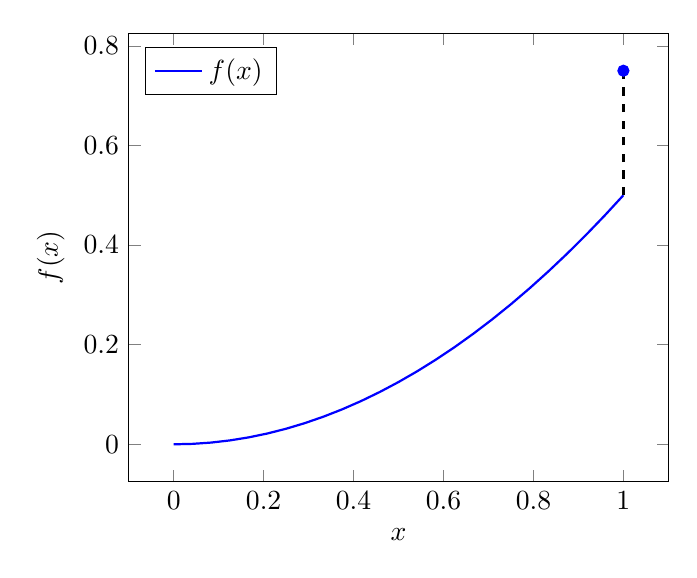
\begin{tikzpicture}% function
        \begin{axis}[xlabel=$x$,ylabel=$f(x)$, legend pos=north west]
        \addplot[thick, color=blue,domain = 0:1] {(0.5 * (x * x))};
        \addplot[mark=*, color=blue] coordinates {(1,0.75)};
        \draw [dashed, very thick] (1,0.5) -- (1,0.75);
        \legend{$f(x)$}
        \end{axis}
        \end{tikzpicture}
        \caption{Graph for $f$ from~\cref{eq:pw-f}}
        \label{fig:pw-f}
    \end{figure}
    \item $g$ is not necessarily closed.
    \end{enumerate}
\end{Exercise}


\begin{Exercise}
	We are given that $f$ is diffable and convex, with $L$-Lipschitz gradient.
	This implies that
	\[
		\abs{\grad f(x) - \grad f(y)} \leq L \norm{x - y}.
	\]
	Additionally, we consider the sequence of points
	\begin{align}
		x_{k+1} = x_k - A_k^{-1} \grad f(x_k) \Rightarrow
		\grad f(x_k) = A_k \left(x_{k} - x_{k+1}\right)
		\label{eq:seq-def}
	\end{align}
	where $A_k$ is a sequence of symmetric matrices satisfying
	$\inf_k \underline{\lambda_k} > \frac{L}{2}, \; \sup_k \overline{\lambda_k}
	< \infty$, where $\underline{\lambda}_k$, $\overline{\lambda}_k$ are the
	smallest and largest eigenvalues of $A_k$, respectively.

	To prove that $\set{x_k}_{k=1}^{\infty}$ is a slope descent sequence, we
	need to verify the two postulates given in lecture. Let us try to verify
	the sufficient decrease condition first: we exploit the fact that $f$ is
	convex and $L$-smooth, which implies that it has the following quadratic
	upper bound:
	\begin{align}
		f(z) &\leq f(x) + \ip{\grad f(x), z - x} + \frac{L}{2} \norm{z - x}^2,
		\label{eq:quad-upper-bound},
	\end{align}
	which was stated in lecture and also proven in the lectures of ORIE 6328.
	If we set $x = x_k, z = x_{k+1}$ in~\cref{eq:quad-upper-bound}, we obtain
	(moving terms around):
	\begin{align*}
		f(x_k) - f(x_{k+1}) &\geq \ip{\grad f(x_k), x_{k} - x_{k+1}}
			- \frac{L}{2} \norm{x_k - x_{k+1}}^2 \\
			&\overset{\cref{eq:seq-def}}{=} \ip{A_k (x_{k} - x_{k+1}), x_k -
		x_{k+1}} - \frac{L}{2} \norm{x_k - x_{k+1}}^2 \Rightarrow \\
			&\geq \inf_k \underline{\lambda_k} \norm{x_k - x_{k+1}}^2
			- \frac{L}{2} \norm{x_k - x_{k+1}}^2,
	\end{align*}
	where we have made use of the variational definition of the smallest
	eigenvalue of a matrix:
	\[
		\underline{\lambda} = \inf_{d \neq 0} \frac{d^\top A d}{d^\top d}
		\Rightarrow d^\top A d \geq \underline{\lambda} \norm{d}^2, \; \forall
		d.
	\]
	Since $\inf_k \underline{\lambda}_k > \frac{L}{2}$, it must hold that
	$\exists \alpha > 0: \alpha = \inf_k \underline{\lambda}_k - \frac{L}{2}$,
	so that we may conclude
	\[
		f(x_k) - f(x_{k+1}) \geq \alpha \norm{x_k - x_{k+1}}^2, \; \forall k
		\in \Nbb,
	\]
	which is precisely the sufficient decrease condition. It remains to show
	that
	\[
		\abs{\grad f}(x_{k+1}) \leq \beta \norm{x_k - x_{k+1}}, \; \forall k.
	\]
	Notice that the Lipschitz bound along with the reverse triangle inequality
	give us
	\[
		\norm{\grad f(x_{k+1})} - \norm{\grad f(x_k)} \leq
		\norm{\grad f(x_{k+1}) - \grad f(x_k)} \leq L \norm{x_{k+1} - x_k}
	\]
	which, combined with~\eqref{eq:seq-def}, implies
	\begin{align*}
		\norm{\grad f(x_{k+1})} &\leq \norm{A_k (x_k - x_{k+1})} + L
		\norm{x_{k+1} - x_k} \leq \sup_k \overline{\lambda}_k \norm{x_{k+1} -
		x_k} + L \norm{x_{k+1} - x_k} \\
		&\leq \left(L + \lambda\right) \norm{x_{k+1} - x_k},
	\end{align*}
	where $\lambda = \sup_k \overline{\lambda}_k$, as our assumptions dictate
	that $\set{A_k}$ are uniformly bounded and $\norm{Ax} \leq \opnorm{A}
	\norm{x}$ when $\norm{\cdot} = \norm{\cdot}_2$. This completes the second
	postulate, since in Exercise 2 we proved that $\abs{\grad f}(x) =
	\norm{\grad f(x)}$ for a differentiable function $f$. Hence
	\[
		\abs{\grad f}(x_{k+1}) \leq \left(L + \lambda\right) \norm{x_{k+1} -
		x_k},
	\]
	and the sequence $\set{x_k}_{k=1}^{\infty}$ is indeed a slope descent
	sequence.
\end{Exercise}

\end{document}
